\subsubsection{DNA, Chromosomes and Genomes} \label{background:biology:dna_chromosomes_and_genomes}
\textit{Deoxyribonucleic acid} (DNA) is a type of molecule that carries the genetic instructions for the development, function, and reproduction of all known living organisms.
The molecule is composed of two connected strands that wind around each other into a double helix shape.
Each strand is made up of a sugar and phosphate backbone, with each sugar carrying one out of four bases, often referred to as \textit{nucleotides}. 
The four DNA nucleotides are: \textit{cytosine}, \textit{guanine}, \textit{adenine} and \textit{thymine}, and they are typically referred to by their abbreviations C, G, A and T respectively.
Furthermore, chemical bonds form between complementary pairs of nucleotides: AT/TA and CG/GC, meaning that A and T, and C and G are complementary. 
The two strands are connected by these bonds formed between these nucleotides.
Since the sequence of nucleotides in one strand is complementary to the other, the two strands do in fact encode the same genetic information.
In other words, by having one strand, the other can be determined by reversing the strand you have and then exchanging each nucleotide by its complement.

DNA is organized into structures called \textit{chromosomes}. 
Humans have 46 chromosomes made up by two sets of 23 chromosomes where each chromosome occurs twice. One is inherited from the male parent and the other is inherited from the female parent.

The \textit{genome} of an organism usually refers to the entirety of an organism's genetic information. 

\begin{figure}[ht!]
\begin{center}
\scalebox{1}{
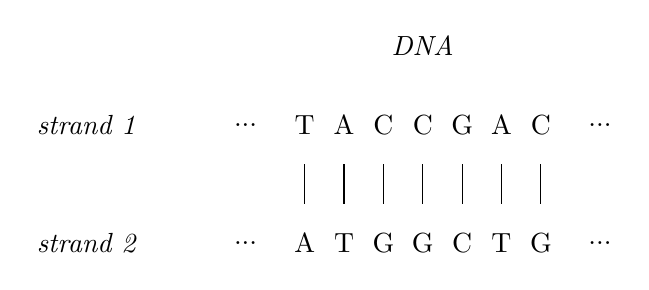
\begin{tikzpicture}
  % texts
  \node at(2.25,2.5)(title){\textit{DNA}};
  \node at(-2,0)(title){\textit{strand 2}};
  \node at(-2,1.5)(title){\textit{strand 1}};
  % lower nodes
  \node at(0,0)(n1){...};
  \node at(.75,0)(n2){A};
  \node at(1.25,0)(n3){T};
  \node at(1.75, 0)(n4){G};
  \node at(2.25,0)(n5){G};
  \node at(2.75,0)(n5){C};
  \node at(3.25,0)(n5){T};
  \node at(3.75,0)(n5){G};
  \node at(4.5,0)(n5){...};
  % upper nodes
  \node at(0,1.5)(n1){...};
  \node at(.75,1.5)(n2){T};
  \node at(1.25,1.5)(n3){A};
  \node at(1.75,1.5)(n4){C};
  \node at(2.25,1.5)(n5){C};
  \node at(2.75,1.5)(n5){G};
  \node at(3.25,1.5)(n5){A};
  \node at(3.75,1.5)(n5){C};
  \node at(4.5,1.5)(n5){...};
  % base pair bonds 
  \draw (.75,.5) -- (.75,1);
  \draw (1.25,.5) -- (1.25,1);
  \draw (1.75,.5) -- (1.75,1);
  \draw (2.25,.5) -- (2.25,1);
  \draw (2.75,.5) -- (2.75,1);
  \draw (3.25,.5) -- (3.25,1);
  \draw (3.75,.5) -- (3.75,1);
\end{tikzpicture}
}
\caption{A conceptual representation of a DNA molecule made up of two strands. The strands are composed of nucleotides forming base pairs where A (adenine) and T (thymine), and C (cytosine) and G (guanine) are complements of each other.}
\label{background:biology:dna_and_chromosomes:figures:dna_strands}
\end{center}
\end{figure}

Studying organisms' DNA is important for a variety of reasons.
It is particularly important to understand genetic diseases and how to best treat them.

...
